\documentclass{article}
\usepackage[utf8]{inputenc}
\usepackage[T1]{fontenc}
\usepackage[french]{babel}
\usepackage[a4paper, margin=2.5cm]{geometry}
\usepackage{amsmath, amssymb, graphicx, xcolor, hyperref}
\usepackage{booktabs}

\begin{document}

\title{Rapport Projet C++ : Donjon interactif}
\author{Amaury JACOB-PIACENTINI}
\date{\today}

\maketitle

\section{Introduction}

Dans ce projet, j'ai codé un labyrinthe interactif en C++. Le code creer un donjon, placer le joueur à une entrée, puis on peut se déplacer dans la map. Mon objectif était de construire un projet structuré, lisible et suffisamment modulaire pour le modifier facilement.

Le jeu fonctionne dans un terminal. À chaque tour, la grille est affichée avec la position du joueur, ses points de vie, son inventaire, la distance jusqu'à la sortie et les déplacements possibles. Le joueur peut se déplacer avec les touches \texttt{w}, \texttt{s}, \texttt{a} et \texttt{d}, ou quitter avec \texttt{x}.

\section{Organisation générale du code}

J'ai séparé le projet en plusieurs fichiers afin d'éviter d'avoir tout le code dans un seul fichier. Le fichier \texttt{main.cpp} contient la boucle principale du jeu et la lecture des commandes du joueur. La classe \texttt{Donjon} gère la grille, la génération du labyrinthe, le placement des éléments, les déplacements et le calcul de la distance jusqu'à la sortie. Les fichiers liés aux cases regroupent les comportements des différents objets présents dans le donjon, tandis que la classe \texttt{Character} représente le joueur, ses points de vie et son inventaire.

\begin{table}[h]
\centering
\begin{tabular}{ll}
\toprule
Fichier & Rôle principal \\
\midrule
\texttt{main.cpp} & Boucle de jeu et saisie utilisateur \\
\texttt{donjon.cpp} / \texttt{donjon.h} & Génération, affichage, déplacements et distance \\
\texttt{case.cpp} / \texttt{case.h} & Implémentation des types de cases \\
\texttt{character.cpp} / \texttt{character.h} & Gestion du joueur \\
\texttt{CMakeLists.txt} & Configuration de compilation \\
\bottomrule
\end{tabular}
\caption{Organisation des fichiers du projet}
\end{table}

J'ai aussi utilisé une petite factory pour centraliser la création des cases. Ce choix évite de répéter les appels aux constructeurs à plusieurs endroits du programme. Quand le donjon doit créer un mur, un passage, un trésor, un piège ou un monstre, il peut passer par la même méthode de création. Cela rend le code plus simple à faire évoluer, car l'ajout ou la modification d'un type de case est plus localisé.

\section{Choix d'implémentation}

Pour générer le labyrinthe, j'ai utilisé un algorithme de \textit{recursive backtracking} comme sugérré dans le sujet. La grille est d'abord remplie de murs puis l'algorithme creuse progressivement des passages en avançant de deux cases et en ouvrant le mur intermédiaire. Ce choix permet d'obtenir un labyrinthe cohérent, avec des chemins connectés, tout en gardant une implémentation assez simple.

Une fois que le donjon est généré j'ajoute des éléments spéciaux sur certaines cases accessibles. Les trésors peuvent être récupérés les pièges retirent des points de vie et les monstres déclenchent un combat. Dans la fonction de déplacement, je teste donc le type de la case cible avant de déplacer réellement le joueur. Cela permet de gérer chaque événement au moment où le joueur entre sur une case.


J'ai également ajouté un calcul de distance jusqu'à la sortie avex le BFS. À partir de la position actuelle du joueur, le programme explore les cases accessibles jusqu'à trouver la sortie. J'utilise un tableau pour marquer les cases visitées et un tableau de parents pour reconstruire le chemin trouvé. Cette distance est ensuite affichée dans les statistiques afin de donner une indication au joueur sur sa progression.

Chaque objet possède un caractère d'affichage, ce qui permet de visualiser rapidement l'état du donjon. J'ai aussi affiché les déplacements possibles afin de rendre le jeu plus clair et d'éviter que le joueur essaye trop souvent de traverser un mur. J'ai décidé d'utilisé wcout pour pouvoir utiliser des characters spéciaux pour les murs.

vous pouvez voir une image du jeu ci-dessous :
\begin{figure}[h]
    \centering
    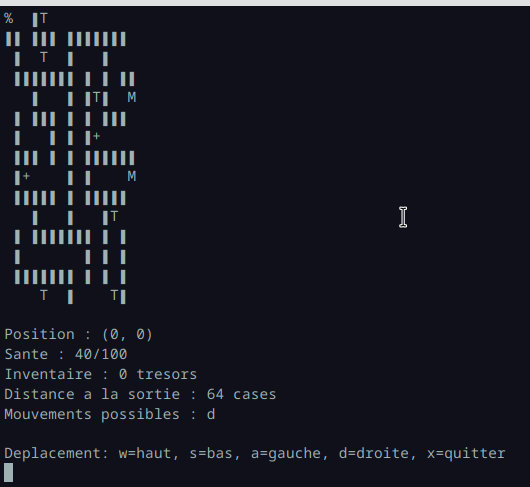
\includegraphics[width=0.7\textwidth]{image.png}
    \caption{Exemple d'affichage du labyrinthe}
    \label{fig:labyrinthe}
\end{figure}
\subsection{Combat}
J'ai aussi implémenté une mécamique très basique de combat contre les monstres. Quand le joueur marche sur une case monstre un combat se déclenche. Le joueur tire un dé 6 pour attaquer et le monstre tire aussi un dé 6. le joueur peut décider de fuir ou d'utilisé un trésor pour regagner des hp. Nomalement il y aurait du avoir différent type de monstre avec des caractéristiques différentes mais je n'ai pas eu le temps de l'implémenter.

\section{Fichiers \texttt{.h} et CMake}

J'ai utilisé des fichiers \texttt{.h} pour séparer les déclarations des classes de leur implémentation. Par exemple, les attributs et les méthodes de \texttt{Donjon} sont déclarés dans \texttt{donjon.h}, tandis que le détail des fonctions est écrit dans \texttt{donjon.cpp}. Cette organisation rend le projet plus lisible, car on peut comprendre rapidement l'interface d'une classe sans lire toute son implémentation.

Pour la compilation, j'ai utilisé CMake avec un fichier \texttt{CMakeLists.txt}. C'est pratique pour un projet composé de plusieurs fichiers \texttt{.cpp}, car cela évite de lancer manuellement une longue commande de compilation. CMake permet aussi de garder une structure plus propre et de recompiler plus facilement le projet sur une autre machine.

Ce projet était une bonne excuse pour pouvoir me former à ca.


Vous pouvez testez de compiler le jeu en faisant :
\begin{verbatim}
    make clean
    make
\end{verbatim}
dans le dossier build.

\section{Difficultés rencontrées}

La principale difficulté a été le calcul de la distance jusqu'à la sortie. Le BFS doit partir de la position actuelle du joueur et non seulement de l'entrée du labyrinthe. Lors d'un débug, j'ai remarqué que le programme pouvait se bloquer après quelques déplacements parce que la reconstruction du chemin ne s'arrêtait pas au bon endroit. J'ai donc corrigé la logique pour que le chemin soit reconstruit jusqu'à la position réelle du joueur.


\section{Utilisation de l'IA générative}

J'ai très peu utilisé l'IA générative pendant le développement du projet. Après 1h à pas trouver un bug je l'ai utiliser. C'était un bug d'importation circulaire, je ne l'aurai jamais trouvé. Je l'ai aussi utilisée pour m'aider à formuler et structurer ce rapport.

Vous pouvez regarder mon github pour mes commit régulier: \url{https://github.com/JacobAmaury/projet_m1_c-_interactif_labyrinthe}

\section{Conclusion}

Ce projet m'a permis de mettre en pratique plusieurs notions importantes de C++ : la programmation orientée objet, l'héritage, le polymorphisme, la séparation en fichiers \texttt{.h} et \texttt{.cpp}, ainsi que la compilation d'un projet multi-fichiers avec CMake. Le résultat obtenu est un jeu de labyrinthe fonctionnel dans le terminal, avec une génération aléatoire, des déplacements, des événements sur les cases, des combats et un calcul de distance jusqu'à la sortie.

Le projet pourrait encore être amélioré, par exemple avec une meilleure gestion de la mémoire, une interface plus avancée ou plusieurs niveaux, mais il répond déjà aux principales fonctionnalités attendues pour un donjon interactif.
\end{document}